\documentclass[pdf, autumn, slideColor, nocolorBG]{prosper}
\usepackage{verbatim}
\usepackage{color}
\usepackage{hyperref}
\usepackage{biblatex}
\usepackage{subfig}

%General Short-Cut Commands
\newcommand{\superscript}[1]{\ensuremath{^{\textrm{#1}}}}
\newcommand{\subscript}[1]{\ensuremath{_{\textrm{#1}}}}
\newcommand{\nuc}[2]{\superscript{#2}{#1}}
\newcommand{\FigCaption}[1]{\begin{center}{\tiny{#1}}\end{center}}

%Commands for this document...
\newcommand{\Red}[1]{\textcolor{red}{#1}}


% Bibliography
\bibliography{../library}{}


%Presentation information
\title{Essential Physics Fuel Cycle Modeling \& Analysis}
\subtitle{PhD Defense - September 7\superscript{th}, 2010 - Austin, TX}
\author{Anthony Scopatz}
\email{scopatz@mail.utexas.edu}
\institution{\tiny
Department of Mechanical Engineering, Nuclear Engineering Program\\
The University of Texas at Austin\\
1 University Station, MC R9000, Austin, TX 78712
}

\slideCaption{Scopatz - PhD Defense}

\begin{document}

% make the title slide
\maketitle


% Motivation
\overlays{5}{
\begin{slide}{Motivation}
\FromSlide{1}
\begin{itemize}
    \item Many nuclear fuel cycle simulations are formulated on premade base-case scenarios:

\FromSlide{2}
    \begin{center}
    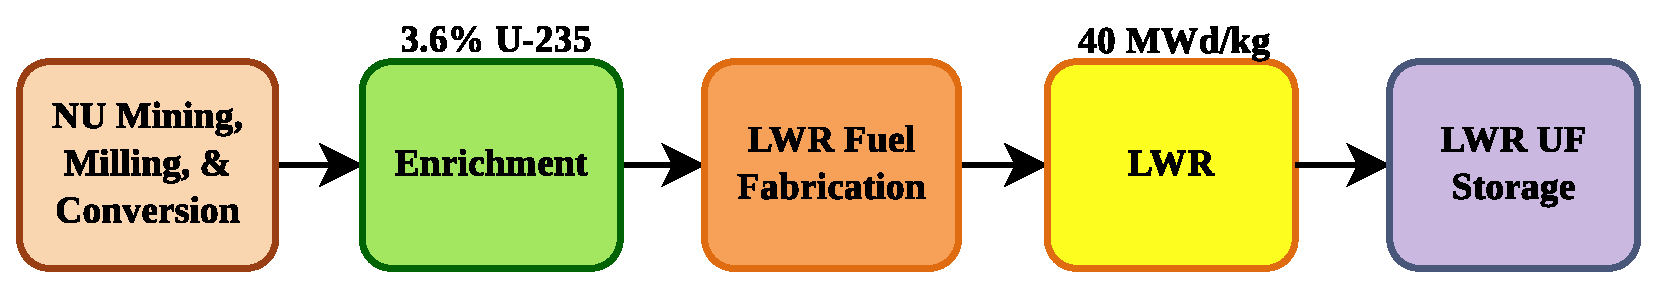
\includegraphics[scale=0.25]{figs/OnceThrough.eps}
    \end{center}

\FromSlide{3}
    \item These base cases are very well studied.

\FromSlide{4}
    \item However, what is \textbf{\textit{not}} well known is 
        how these sample scenarios are affected by perturbations to their 
        initial physical parameters.
            
\FromSlide{1}
\end{itemize}

\FromSlide{5}
\begin{center}
``\textit{Do our parameter choices really give us the `best' solution?}''
\end{center}

\end{slide}}


% Motivation
\begin{slide}{Motivation}
\begin{center}
\begin{figure}
\caption{Physics Modeled versus Execution Time}
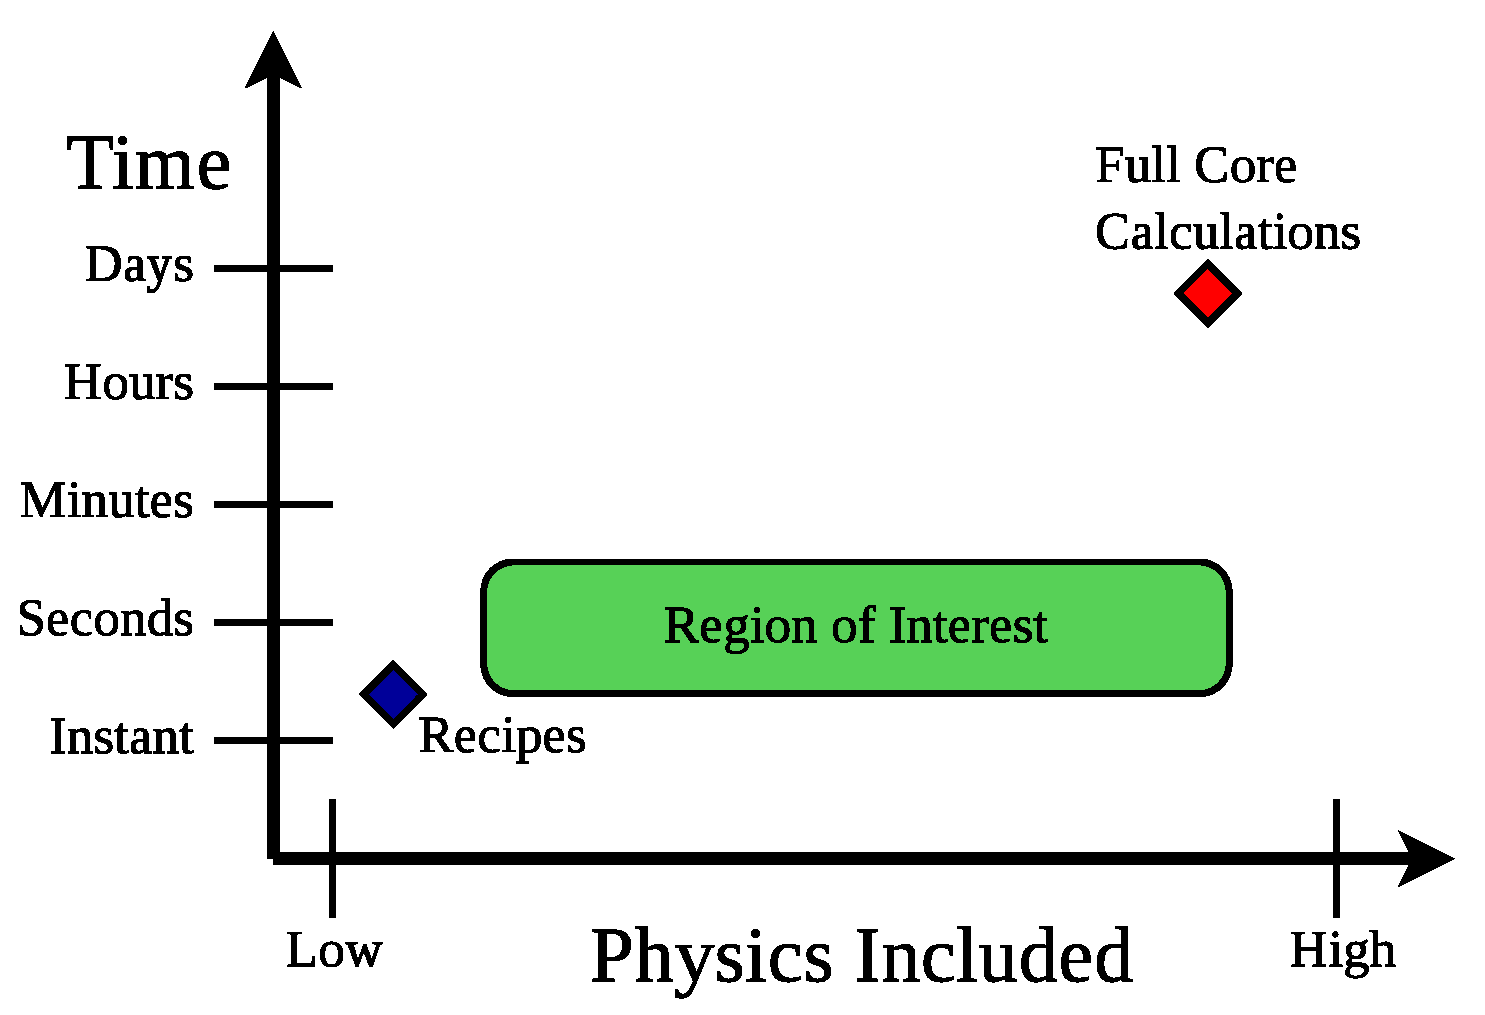
\includegraphics[scale=0.35]{figs/physics_vs_exec_time.eps}
\end{figure}
\end{center}
\end{slide}



% Motivation
\overlays{2}{
\begin{slide}{Motivation}
\FromSlide{1}
\begin{itemize}
    \item Investigating the region of interest may provide a 
        \textit{transformative} amount of fuel cycle data.  

\FromSlide{2}
    \item However, this requires an entirely new spectrum of tools.

\FromSlide{1}
\end{itemize}


\FromSlide{2}
\setcounter{figure}{1}
\begin{center}
\begin{figure}
\caption{Fuel Cycle Stack}
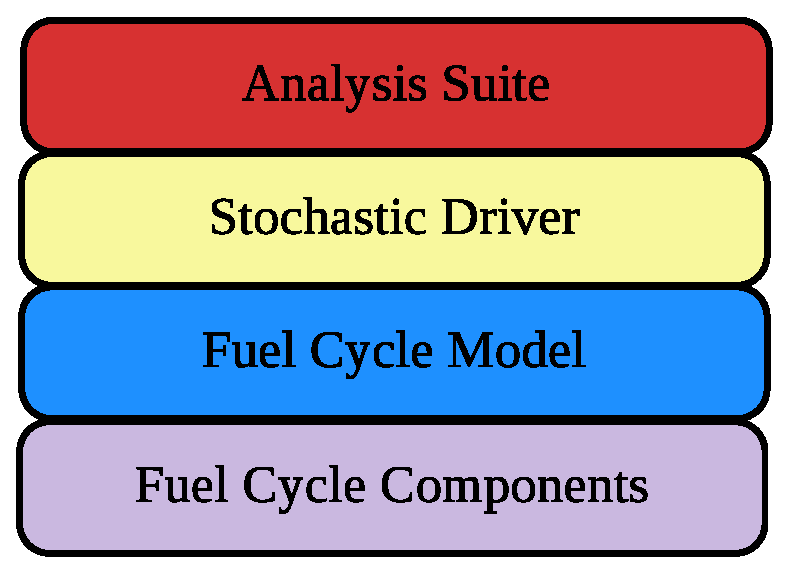
\includegraphics[scale=0.35]{figs/fc_stack.eps}
\end{figure}
\end{center}

\end{slide}}



% Definition
\begin{slide}{Definition}
\vspace{3.0cm}
\begin{center}
\textit{Essential physics} models remain physically valid under perturbations
in the locality of the region that they are defined and do not compute
extraneous parameters.  
\end{center}
\end{slide}




% A Path Forward
\overlays{4}{
\begin{slide}{A Path Forward}
\FromSlide{1}
\begin{itemize}
    \item Develop a set of fuel cycle component models which 
        preserve basic physics (largely focused on a one-enegy 
        group reactor model, R1G).

\FromSlide{2}
    \item Investigate a categorical set of fuels cycles using
        the above components. (These are largely linear 
        perturbations of previous base-case studies.)

\FromSlide{3}
    \item Extend the fuel cycle model to perturb continuous 
        variables.  This requires a stochastic driving mechanism
        to run.  Moreover, it requires entropy-based measures to
        analyze.

\FromSlide{4}
    \item Model the reactor compoent with 
        multiple energy groups (RMG).  This enables the study 
        of reactors and fuel cycles forbidden in the R1G regime.

\FromSlide{1}
\end{itemize}
\end{slide}}




% R1G
\begin{slide}{R1G}
\vspace{3.5cm}
\begin{center}
\Large
One-Group Reactor Model
\end{center}
\end{slide}





% R1G
\begin{slide}{R1G}
\begin{center}
\begin{figure}
\caption{Reactor Model [1]}
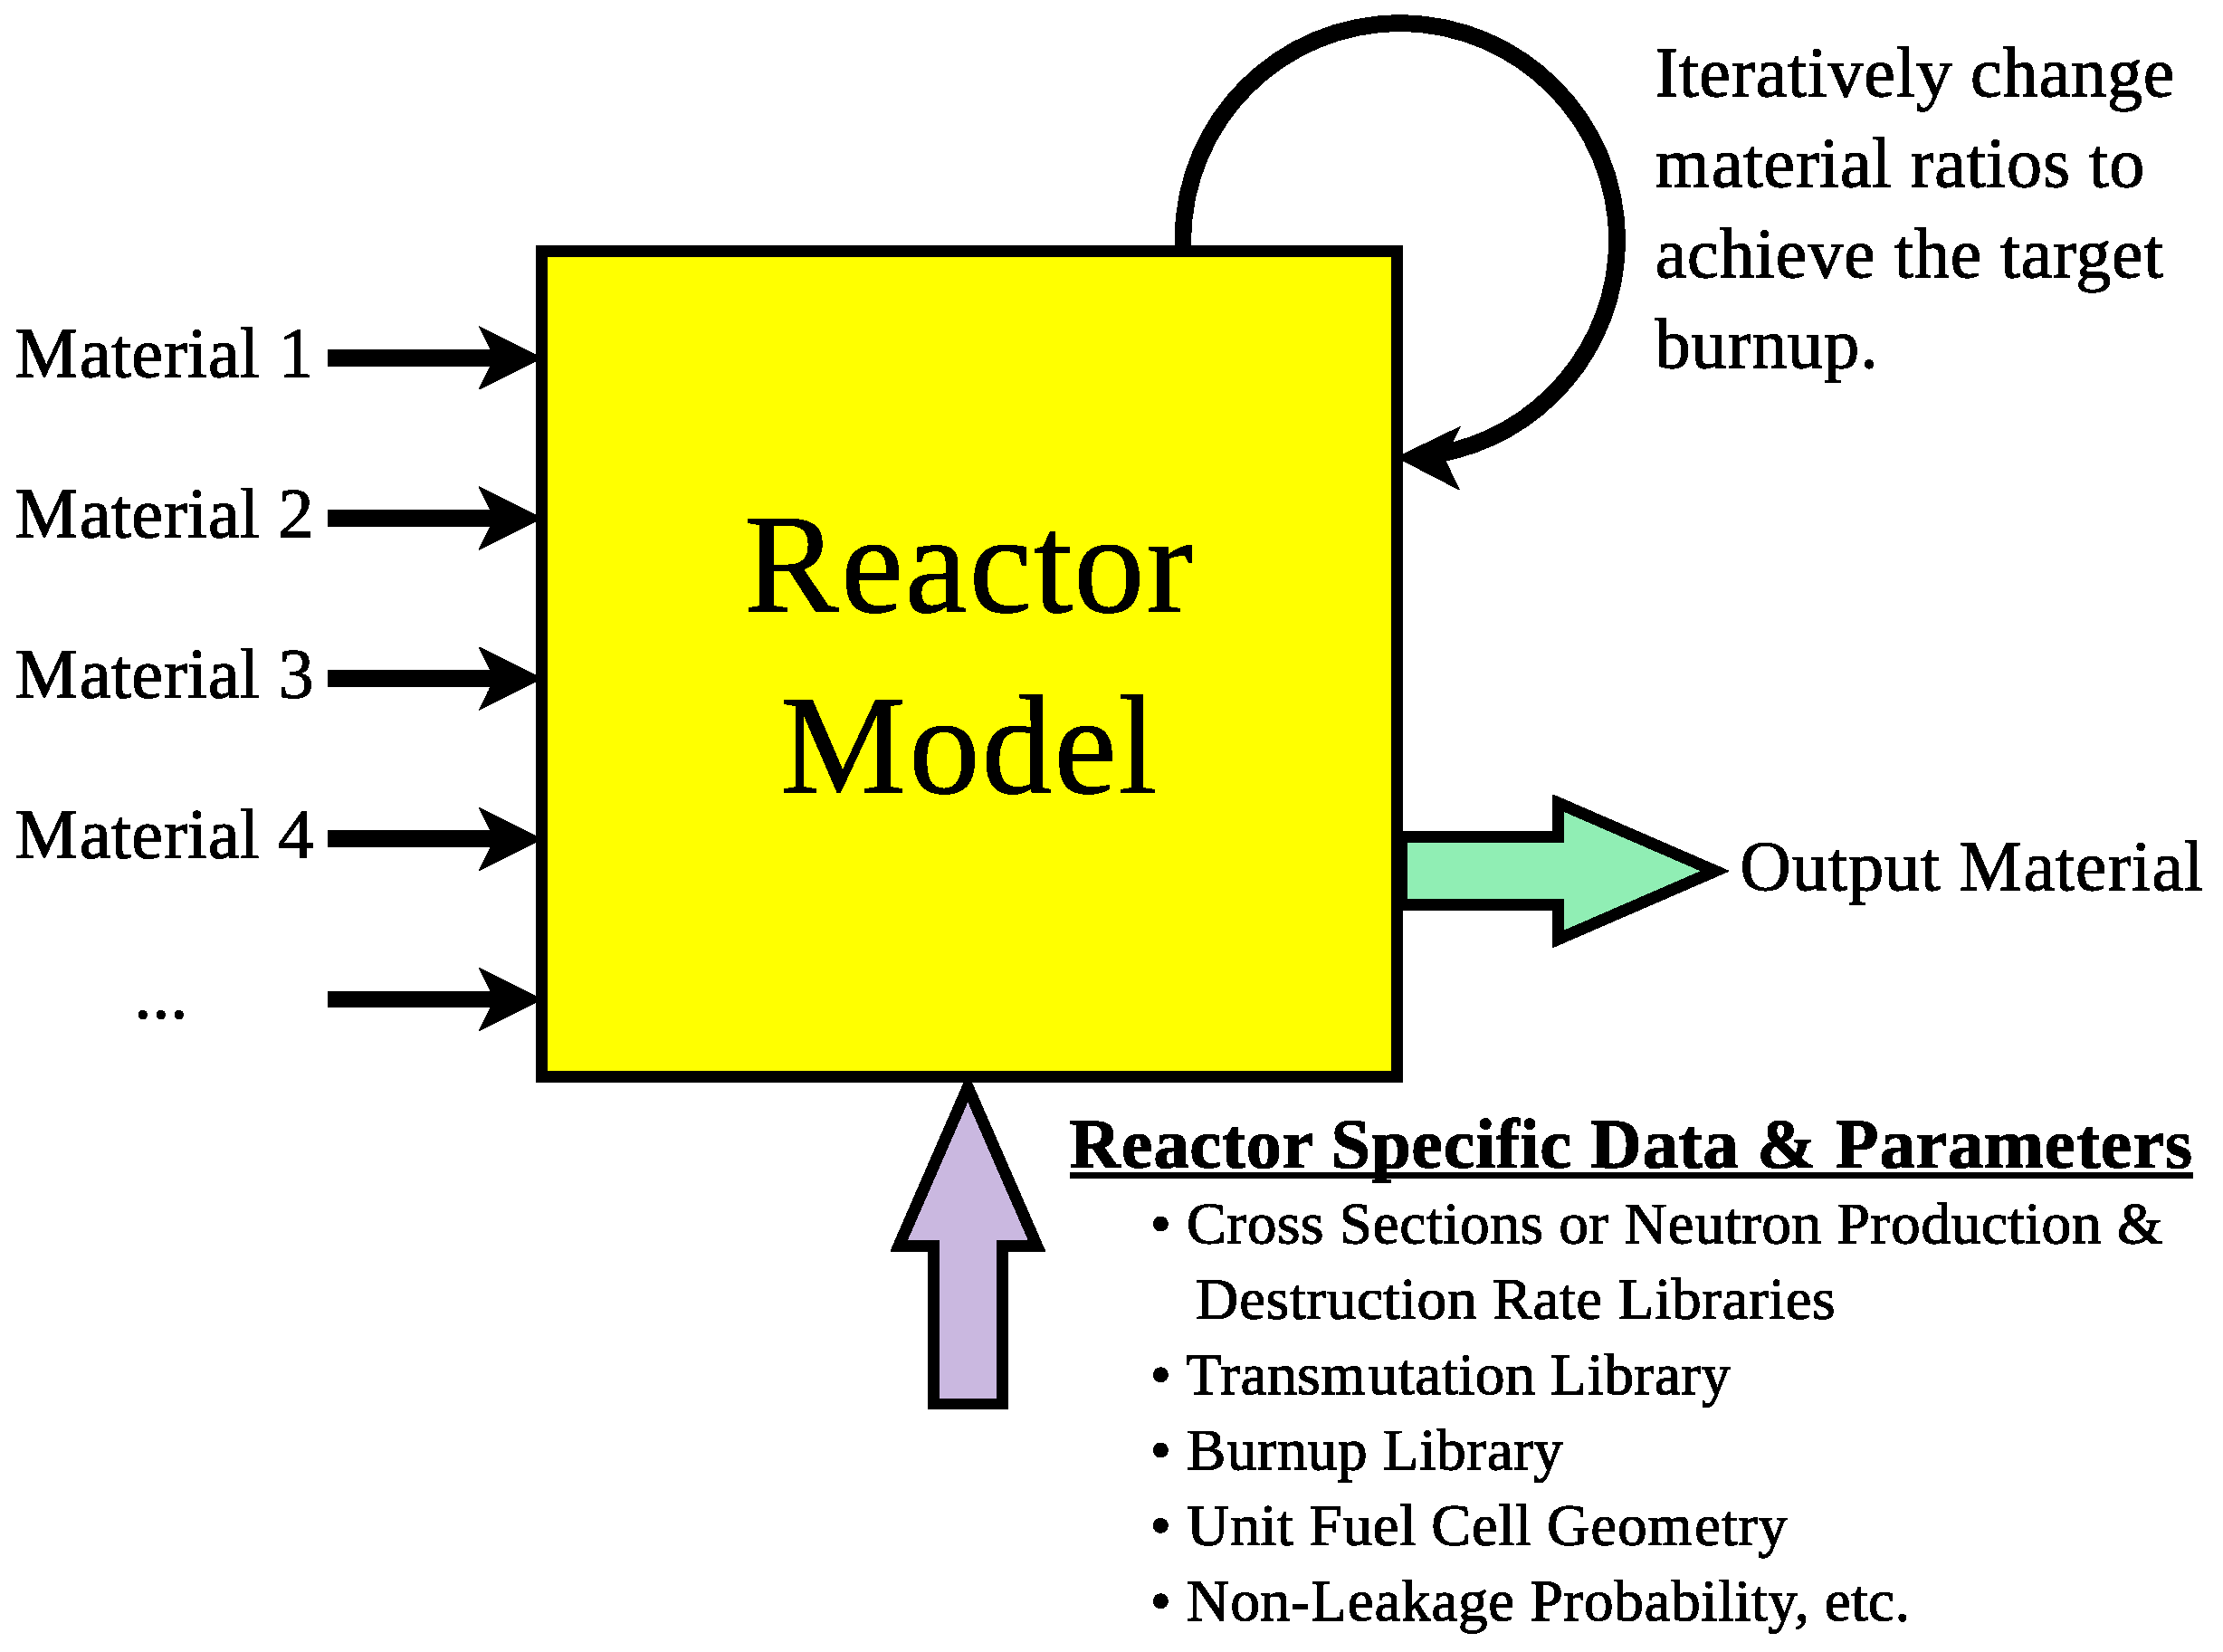
\includegraphics[scale=0.20]{figs/reactor_model.eps}
\end{figure}
\end{center}
\end{slide}



% R1G Notation
\begin{slide}{R1G Notation}
\vspace{0.75cm}
\begin{center}
\begin{table}
\caption{One-Group Reactor Symbols}
\tiny
\begin{tabular}{|l|c|c|}
\hline
\textbf{Name} & \textbf{Symbol} & \textbf{Units} \\
\hline
Fluence & $F = \int_0^t \phi dt^\prime = \phi \int_0^t dt^\prime = \phi \times t \cdot \frac{24 \cdot 3600 \cdot 10^3}{10^{24}}$ & [n/kb] \\
Nuclide Subscript & $i$ (or $j$) & [1/kg\subscript{$i$}] \\
Region Superscript & $Q$ & [unitless] \\
Mass Weights & $m_i^Q = \frac{N_i^Q}{N_{\mbox{IHM}}} = \frac{n_i^Q A_i}{A_{\mbox{IHM}}} \cdot \frac{\rho^Q\cdot\mbox{MW}^F}{\rho^F\cdot\mbox{MW}^Q} \frac{V^Q}{V^F}$ & [kg$_i^Q$/kgIHM] \\
Burnup & $\mbox{BU}(F) = \sum_i m_i^F \cdot \mbox{BU}_i(F)$ & [MWd/kgIHM] \\
Prod \& Des Rates & $p_i(F), d_i(F)$ & [n/s/flux/kg$_i$]\\ 
Transmutation Matrix & $T_{ij}(F)$ & [kg$_j$/kg$_i$] \\
Multiplication Factor & $k(F) = \frac{P(F)}{D(F)}$ & [unitless] \\
\hline
\end{tabular}
\end{table}
\end{center}
\end{slide}





% R1G
\overlays{2}{
\begin{slide}{R1G}
\FromSlide{1}
\begin{center}
Starting with ORIGEN generated fluence-dependent, nuclide specific data, we know:

\setcounter{figure}{3}
\begin{figure}
\subfloat[prod \& des rates,]{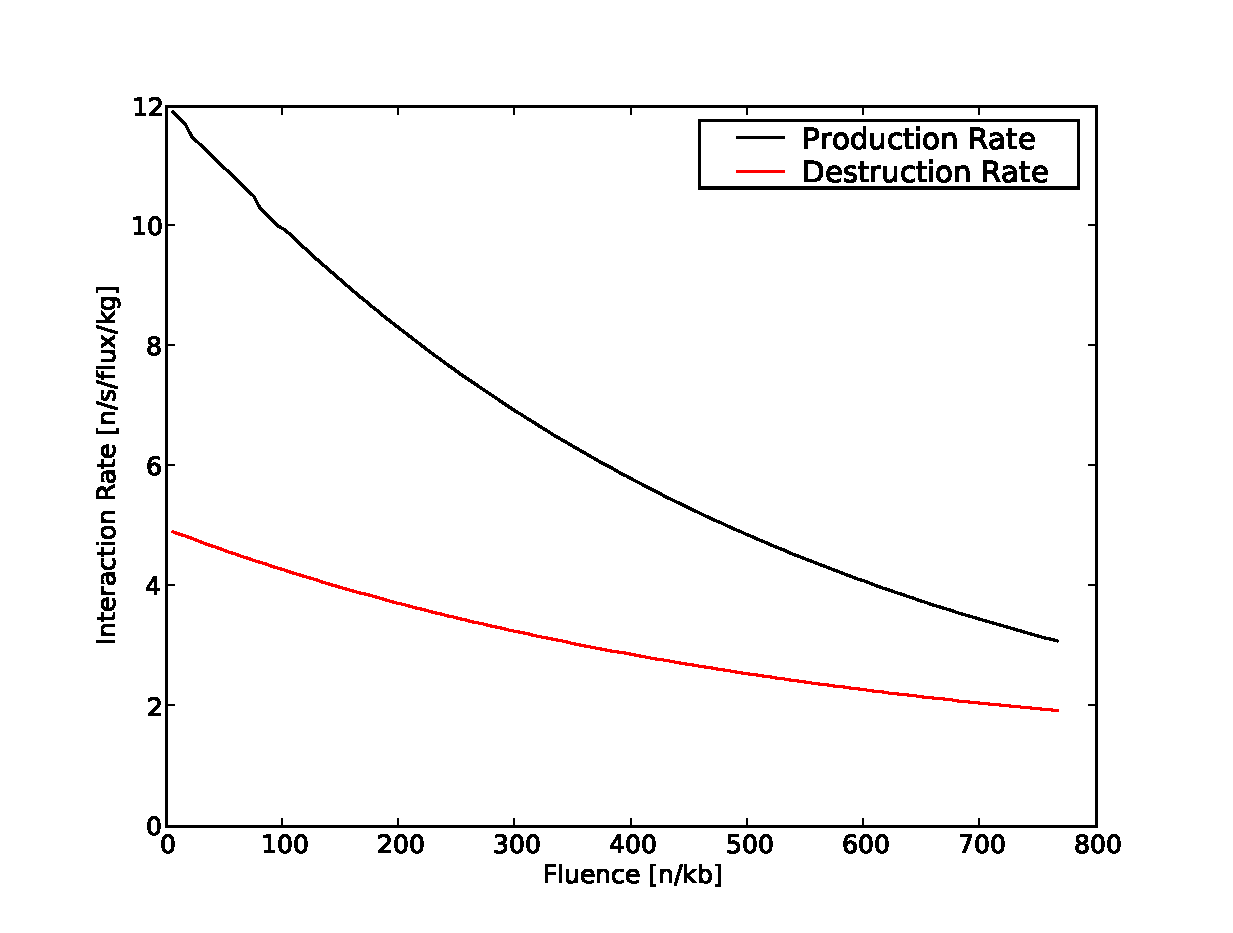
\includegraphics[scale=0.21]{../one_group_method/figs/Fig02.eps}}
\subfloat[burnups,]{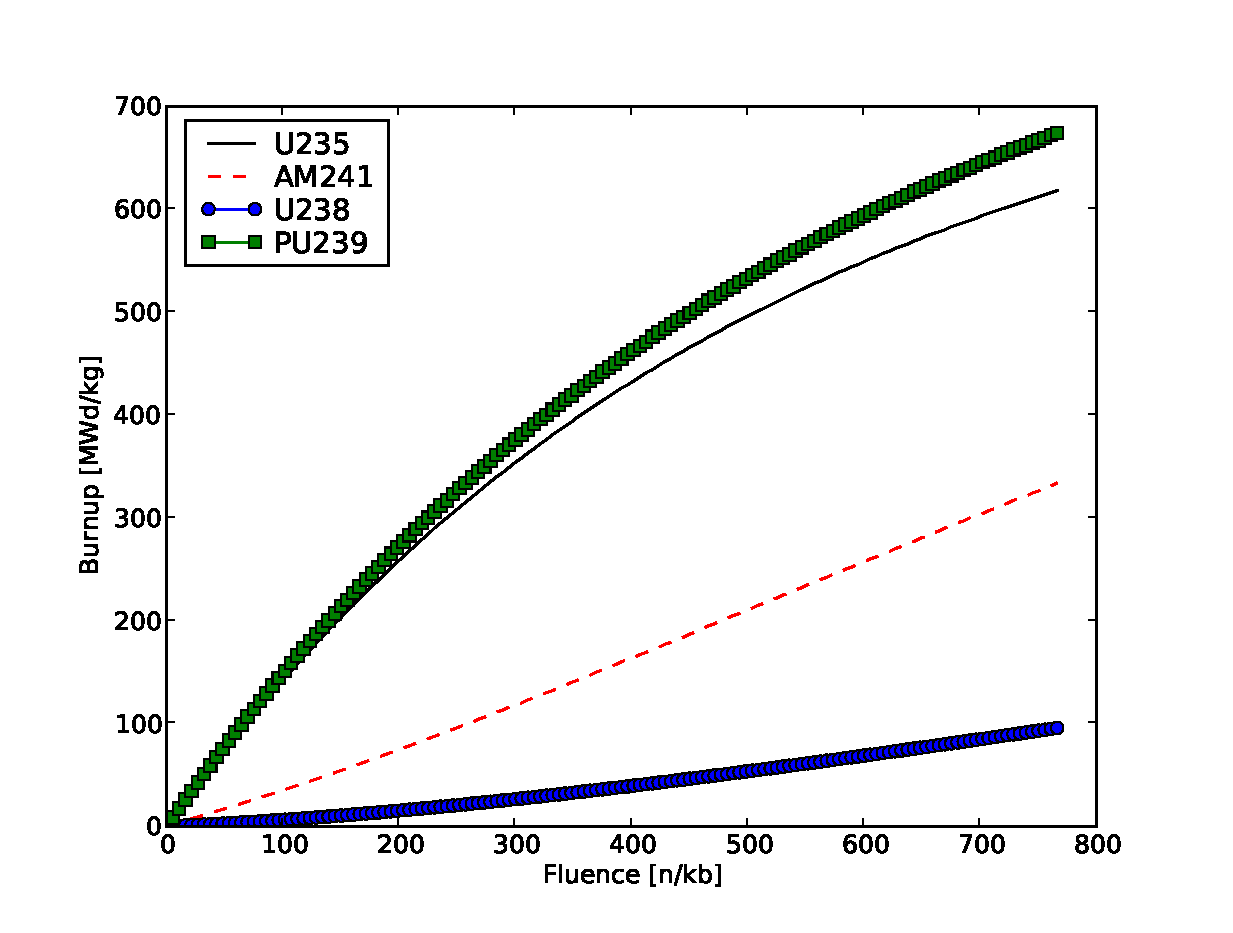
\includegraphics[scale=0.21]{../one_group_method/figs/Fig03.eps}}
\subfloat[transmutation matrices.]{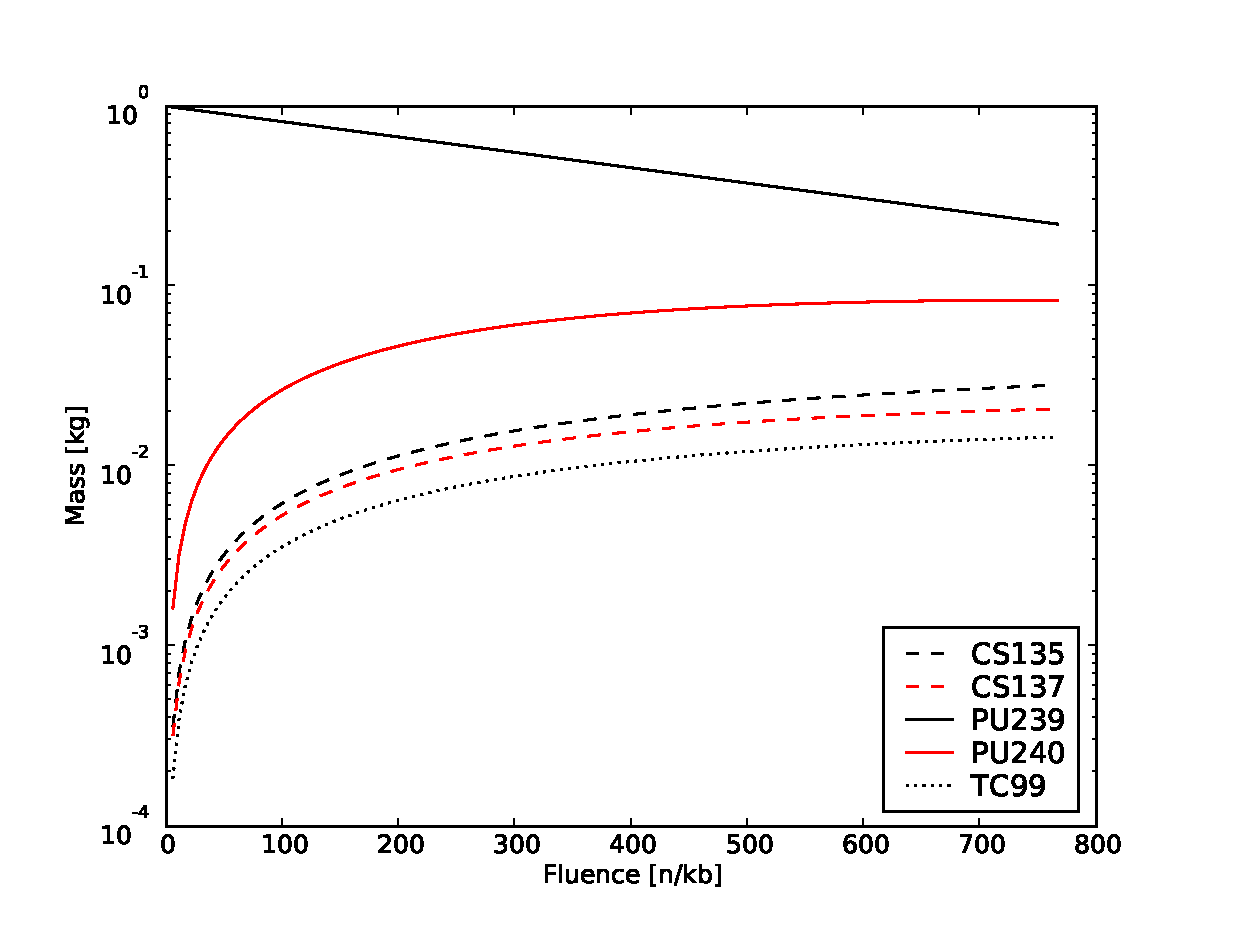
\includegraphics[scale=0.21]{../one_group_method/figs/Fig01.eps}}
\caption{Reactor Data Library (for FR \nuc{Pu}{239})}
\end{figure}

\end{center}

\FromSlide{2}
\footnotesize
Folding these together based on an initial material yields...
\end{slide}}





% R1G
\begin{slide}{R1G}
\begin{center}
\begin{figure}
\caption{Linearly Weighted Fast Reactor Data}
\subfloat[Burnup]{\includegraphics[scale=0.31]{../one_group_method/figs/Fig05.eps}}
\subfloat[Multiplication Factor]{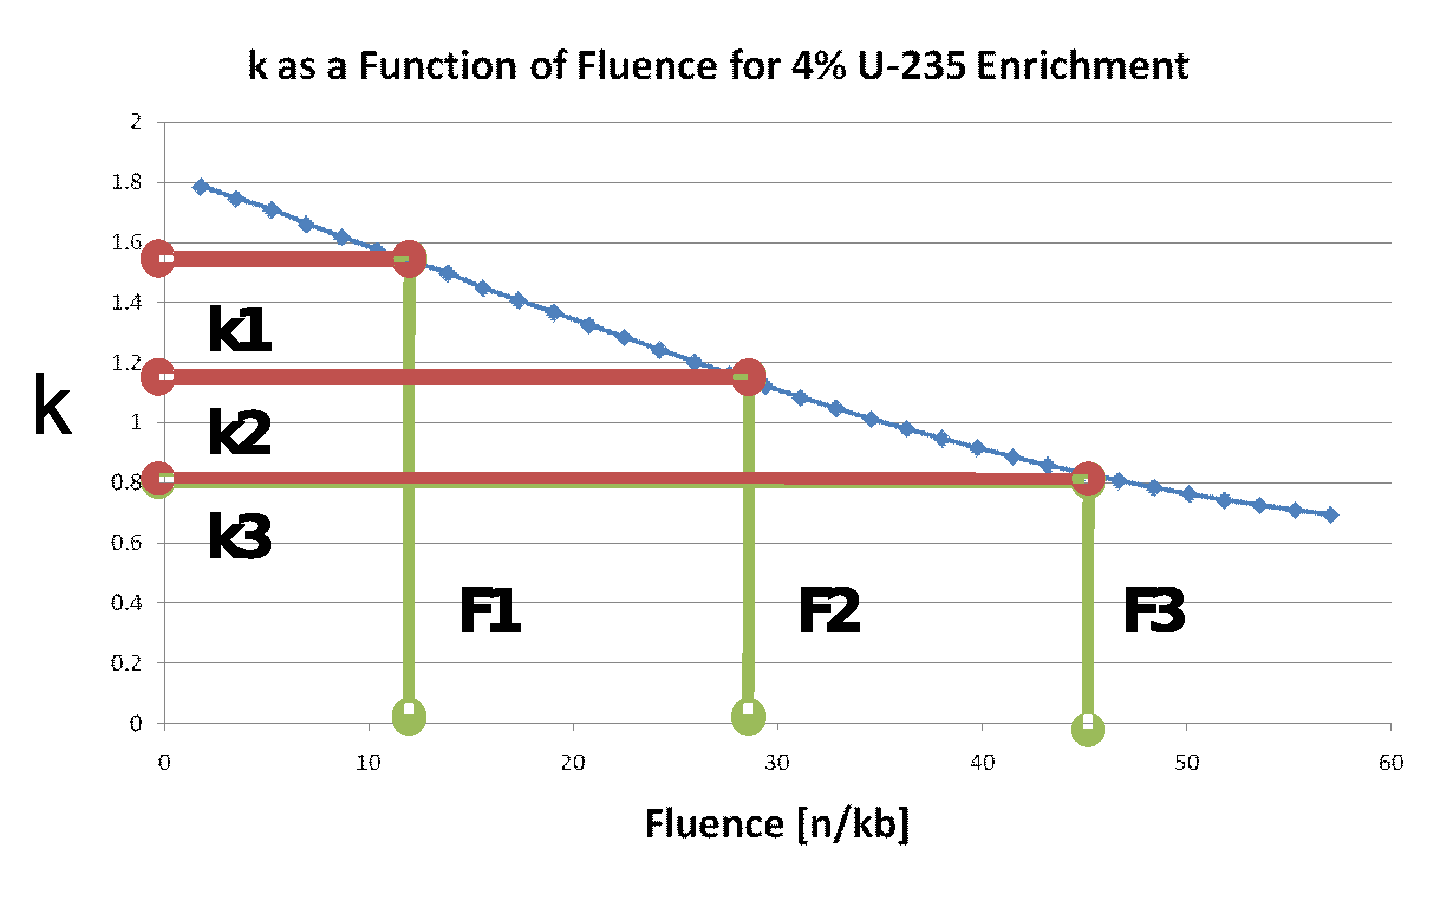
\includegraphics[scale=0.31]{../one_group_method/figs/Fig06.eps}}
\end{figure}
\end{center}
\end{slide}



% R1G 
\overlays{3}{
\begin{slide}{R1G}
\FromSlide{1}
\begin{minipage}[t]{0.49\textwidth}
\setcounter{figure}{5}
\begin{figure}
\caption{Fast Reactor\\ Discharge Composition}
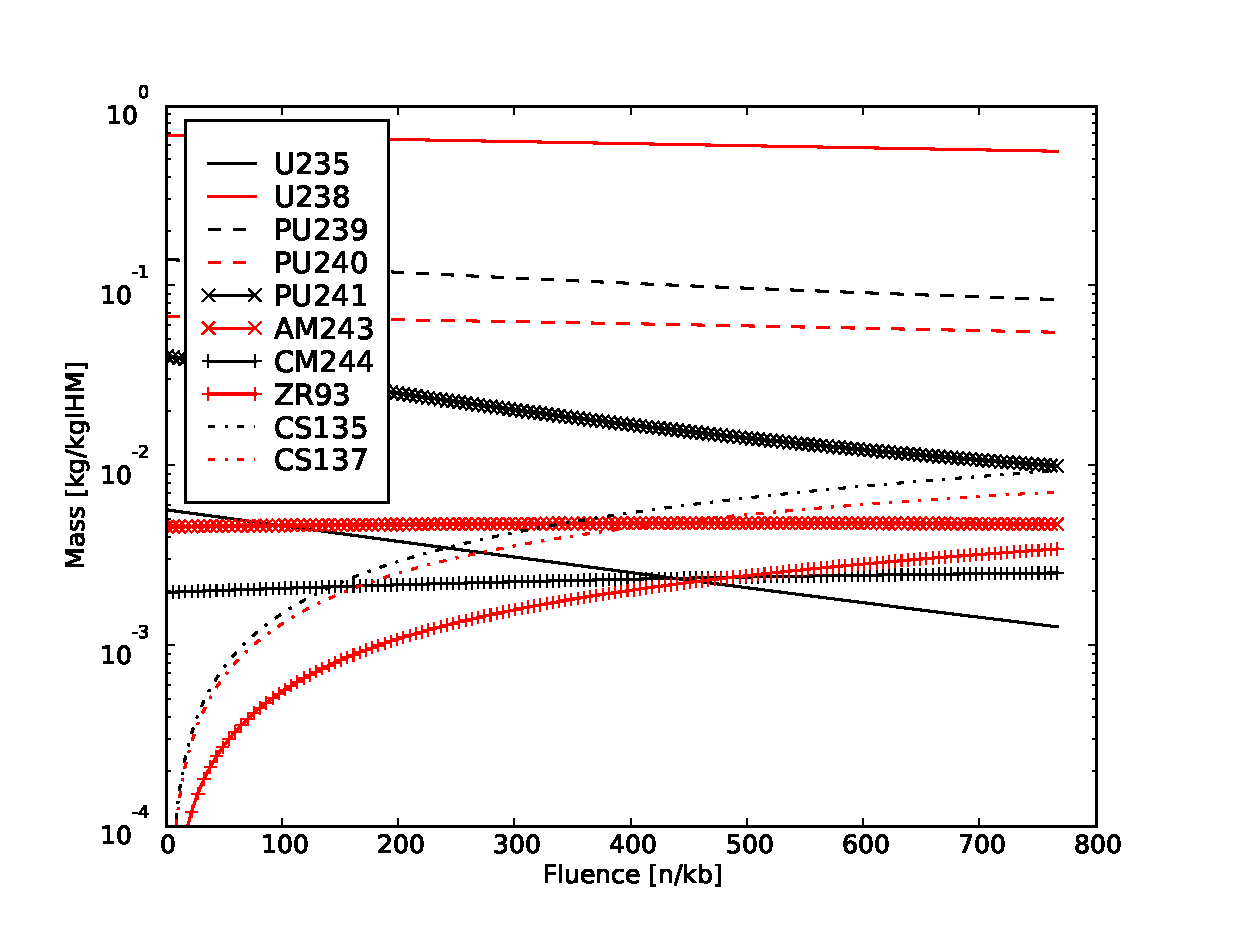
\includegraphics[scale=0.3]{../one_group_method/figs/Fig07.eps}
\end{figure}
\end{minipage}
\begin{minipage}[t]{0.49\textwidth}
\small
\begin{itemize}
    \item The transmutation matrices may be similarly weighted by inital composition.

\FromSlide{2}
    \item From the criticality calculation above we also know the discharge fluence, Fd [n/kb].

\FromSlide{3}
    \item Therefore the used fuel composition is known by taking the nuclide mass weights at 
            Fd in Figure 6.

\FromSlide{1}
\end{itemize}
\end{minipage}
\end{slide}}




% R1G Benchmark
\begin{slide}{R1G Benchmark}
\tiny
\begin{table}[htbp]
\begin{center}
\caption{LWR Benchmark to OECD Burnup Credit [2]}
\begin{tabular}{|l|c|c|c|c|}
\hline
\textbf{Nuclide} & \textbf{OECD [2] [w/o]} & \textbf{$\sigma$ of OECD [\%]} & \textbf{Results [w/o]} & \textbf{\% Difference} \\
\hline
\nuc{U}{234}     & 0.0178  & 9.0  & 0.0184  & +3.6  \\
\nuc{U}{235}     & 0.8001  & 8.1  & 0.7079  & -11.5 \\
\nuc{U}{236}     & 0.4840  & 2.6  & 0.4781  & -1.2  \\
\nuc{U}{238}     & 93.3333 & 0.2  & 93.6109 & +0.3  \\
\nuc{Np}{237}    & 0.0614  & 9.4  & 0.0584  & -5.0  \\
\nuc{Pu}{238}    & 0.0226  & 13.9 & 0.0185  & -18.1 \\
\nuc{Pu}{239}    & 0.5991  & 7.1  & 0.5104  & +14.8 \\
\nuc{Pu}{240}    & 0.2389  & 5.3  & 0.2591  & +8.5  \\
\nuc{Pu}{241}    & 0.1636  & 6.9  & 0.1445  & -11.7 \\
\nuc{Pu}{242}    & 0.0602  & 8.4  & 0.0563  & -6.5  \\
\nuc{Am}{241}    & 0.0047  & 5.3  & 0.0032  & -30.8 \\
\nuc{Am}{243}    & 0.0148  & 10.4 & 0.0116  & -21.3 \\
\hline
\end{tabular}
\end{center}
\end{table}
\end{slide}



% R1G Bechmark Notes
\overlays{2}{
\begin{slide}{R1G Bechmark Notes}
\FromSlide{1}
\begin{itemize}
    \item This benchmark compares an OECD study for a 40 MWd/kgIHM burn with no cooling.

    \item This result shows the R1G matches the burnup credit to within two standard 
        deviations for most actinides.

\FromSlide{2}
    \item \nuc{Am}{241} is the only nuclide showing a relatively higher departure.

    \item This sepcies is formed through \nuc{Pu}{241} decay.

    \item \nuc{Am}{241} would thus match better if a constant flux or 
        if zero reloading times were not assumed.

\FromSlide{1}
\end{itemize}
\end{slide}}




%Methodology Overview
\overlays{4}{
\begin{slide}{Methodology Overview}
\FromSlide{1}
\begin{itemize}
    \item Here, we quantify the system-wide impact of physical parameter perturbations.

\vspace{0.5cm}
\FromSlide{2}
    \item This is done by looking for linear, 1D sensitivity coefficients for each parameter
        to the \underline{repository capacity} response, measured in [PWh].   

\vspace{0.5cm}
\FromSlide{3}
    \item Denote these sensitivity coefficients as $S_x$ for a small change in an input parameter $x$.

\vspace{0.5cm}
\FromSlide{4}
    \item Sensitivity coefficients are presented for 10\% 
        changes in $x$ from assumed base-case values.

\FromSlide{1}
\end{itemize}
\end{slide}}

%Methodology Overview
\overlays{5}{
\begin{slide}{Methodology Overview}
\FromSlide{1}
\begin{itemize}
\FromSlide{1}
    \item The basic algorithm is as follows:

\tiny
\FromSlide{2}
        \begin{enumerate}
            \item For each input parameter $x$, change its base-case value $x_0$ by $\pm10\%$.
                \[ x \to (1 \pm 0.1)x_0 \]

            \FromSlide{3}
            \item If $x$ is a separation efficiency (SE), instead perturb by $\pm$ ``one nine''
                worth of separations.
                \[ x = 0.999 \to x \in \{0.99, 0.9999\} \]

            \FromSlide{4}
            \item Meanwhile, maintain all other parameters ($y, z, \ldots$) at their
                base-case values.
                \[ y, z, \ldots \to y_0, z_0, \ldots \]    

            \FromSlide{5}
            \item Calculate the new repository capacity response, $R$, by the perturbed cycle and record 
                the sensitivity as the percent change from the base-case response, $R_0$.
                \[ S_{\pm x} = \left(\frac{R}{R_0} - 1\right) \times 100 \]

        \FromSlide{2}
        \end{enumerate}

\FromSlide{1}
\end{itemize}
\end{slide}}



%Background
\overlays{2}{
\begin{slide}{Background}
\FromSlide{1}
\begin{itemize}
    \item We have developed a physics-based fuel cycle model
        and used it to study a Fast Reactor (FR), Light
        Water Reactor (LWR) symbiotic scenario 
        analogous to Scheme 3a of the 2006 OECD report.
\end{itemize}

\FromSlide{2}
\begin{center}
\includegraphics[scale=0.65]{figs/FC.eps}
\FigCaption{Figure 1: FR-LWR Cycle}
\end{center}
\end{slide}}




%Background
\overlays{3}{
\begin{slide}{Background}
\FromSlide{1}
\begin{itemize}
    \item In our model, we may adjust over 30 independent physical 
        parameters in the fuel cycle.
\end{itemize}

\FromSlide{2}
\begin{center}
\includegraphics[scale=0.5]{figs/FC_knobs.eps}
\FigCaption{Figure 2: FR-LWR Cycle with Parameter Representation}
\end{center}

\FromSlide{3}
\begin{itemize}
    \item We present equilibrium results derived from a full treatment
        of the preceeding, transient cycles.
\end{itemize}

\end{slide}}


%Reactor Model [1]
\begin{slide}{Reactor Model [1]}
\vspace{0.5cm}

\includegraphics[scale=0.45]{figs/ReactorModel.eps}
\vspace{0.5cm}

\tiny
\textcolor{gray}{\underline{1:} A. M. Scopatz, E. A. Schneider, ``\textit{A New Method for Rapid Computation of 
Transient Fuel Cycle Material Balances,}'' Nuclear Engineering and Design (2009).}
\end{slide}




%Repository Model 
\overlays{2}{
\begin{slide}{Repository Model}
\FromSlide{1}
Like the reactor model, our repository model uses an isotopically weighted linear combination of 
precomputed values that are stored in a data library.

\FromSlide{2}
\begin{center}
\includegraphics[scale=0.50]{figs/RepositoryModel1.eps}
\end{center}

This data library is based off of an infinite series of linear heat sources.  
This is because a repository is constrained by intrinsic temperature limits at 
the driftwall and midway between the drifts.
\end{slide}}





%Repository Model [2]
\begin{slide}{Repository Model [2]}
\vspace{0.5cm}

\includegraphics[scale=0.50]{figs/RepositoryModel2.eps}
\vspace{0.5cm}

\tiny
\textcolor{gray}{\underline{2:} Li, J., Yim, M.-S., McNelis, D., 2004. 
``\textit{Risk-based performance index for nuclear waste transmutation system optimization,}'' 
Trans. Am. Nucl. Soc. 90, 239-240.}
\end{slide}




%Repository Temperature Distribution 
\begin{slide}{Repository Temp Distribution}
\begin{center}
\includegraphics[scale=0.60]{figs/RepositoryModel3.eps}
\end{center}
\end{slide}




%Fuel Cycle Benchmark
\overlays{4}{
\begin{slide}{Fuel Cycle Benchmark}
\FromSlide{1}
\begin{itemize}
    \item We have benchmarked the model on three primary levels: the reactor components, 
        the repository component, and the fuel cycle as a whole.

\FromSlide{2}
    \item LWRs and FRs benchmarks may be found at 
        {\tiny \url{http://nukestar.me.utexas.edu/scopatz/Bright/}}

\FromSlide{3}
    \item For benchmarks of repository performance, see [3].

\FromSlide{4}
    \item However, since the fuel cycle we are modeling is based off of
        the NEA Scheme 3a, we compared our code to the OECD's own results [4].

\FromSlide{1}
\end{itemize}

\FromSlide{4}
\tiny
\textcolor{gray}{\underline{3:} Li, J., Nicholson, M., Proctor,W.C., Yim, M.-S., McNelis, D.N., 2007. 
``\textit{Examining repository loading options to expand yucca mountain repository capacity.}'' 
In: Proc. Advanced Nuclear Fuel Cycles and Systems, GLOBAL, Boise, ID, September.}

\textcolor{gray}{\underline{4:} Nuclear Energy Agency, ``\textit{Advanced Nuclear Fuel 
Cycles and Radioactive Waste Management,}'' - NEA-5990. 2006:1-248.}
\end{slide}}


%Fuel Cycle Benchmark
\begin{slide}{Fuel Cycle Benchmark}
\tiny
\begin{center}
\FigCaption{Table 1: NEA Scheme 3a Benchmark}
\begin{tabular}{|l||c||c|c||c|c|}
\hline
\textbf{Scheme 3a}     & \textbf{NEA} & \textbf{Model\superscript{1}} & \textbf{\% Diff} & \textbf{Model\superscript{2}} & \textbf{\% Diff} \\
\hline
Electricity Share: LWR & 0.632       & 0.619459             & -2.0244 & 0.634907             & +0.4579 \\
\hline
Electricity Share: FR  & 0.368       & 0.380541             & +3.2955 & 0.365093             & -0.7962 \\
\hline
FR SNF: U              & 0.698       & 0.713806             & +2.2143 & 0.715224             & +2.4082 \\
\hline
FR SNF: NP             & 0.0065      & 0.00661961           & +1.8070 & 0.00685174           & +5.1335 \\
\hline
FR SNF: PU             & 0.266       & 0.248059             & -7.2327 & 0.248319             & -7.1204 \\
\hline
FR SNF: AM             & 0.02        & 0.0226796            & 11.8152 & 0.0217317            & +7.9687 \\
\hline
FR SNF: CM             & 0.0098      & 0.00883517           & -10.920 & 0.00787319           & -24.4730\\
\hline
HLW: U                 & 0.013324    & 0.0132681            & -0.4213 & 0.0134448            & +0.8984 \\
\hline
HLW: NP                & 2.26542E-05 & 2.4079E-05           & +5.9173 & 2.41083E-05          & +6.0316 \\
\hline
HLW: PU                & 0.000704797 & 0.000658893          & -6.9668 & 0.000632361          & -11.4548\\
\hline
HLW: AM                & 5.03426E-05 & 5.63068E-05          & 10.5923 & 5.12344E-05          & +1.7405 \\
\hline
HLW: CM                & 2.18151E-05 & 1.99031E-05          & -9.6068 & 1.67094E-05          & -30.5563\\
\hline
HLW: FP                & 0.985876    & 0.985973             & +0.0098 & 0.985831             & -0.0046 \\
\hline
\end{tabular}
\end{center}

1: Model with initial LWR \nuc{U}{235} enrichment of 4.2 w/o. 

2: Model with LWR discharge burnup of 50 MWd/kg.
\end{slide}



\begin{slide}{Sensitivity Results}

\small
\begin{center}
\FigCaption{Table 2: Top Parameters from Screening Study}
\begin{tabular}{|l|c|c|c|}
\hline
\textbf{Parameter $x$}        & \textbf{Base Case $x_0$}    & \textbf{$S_{-x}$} [\%] & \textbf{$S_{+x}$} [\%]\\
\hline
\Red{\texttt{FR\_SE\_PU}}     & \Red{0.999}                 & \Red{-83.09}      & \Red{+99.30} \\
\hline
\Red{\texttt{LWR\_SE\_PU}}    & \Red{0.999}                 & \Red{-60.90}      & \Red{+18.28} \\
\hline
\Red{\texttt{FR\_SE\_AM}}     & \Red{0.999}                 & \Red{-59.53}      & \Red{+17.55} \\
\hline
\Red{\texttt{FR\_SE\_CM}}     & \Red{0.999}                 & \Red{-11.15}      & \Red{+1.28}  \\
\hline
\texttt{FR\_TRU\_CR}          & 0.500                       & +5.22             & -6.02  \\
\hline
\texttt{Rock\_Density}        & 2580 [kg/m\superscript{3}]  & -5.05             & +5.59  \\
\hline
\texttt{Rock\_Specific\_Heat} & 840 [J/kg/K]                & -4.90             & +5.59  \\
\hline
\texttt{LWR\_BUd}             & 50 [MWd/kg]                 & +5.46             & -3.48  \\
\hline
\texttt{FR\_BUd}              & 140 [MWd/kg]                & -5.44             & +5.32  \\
\hline
\end{tabular}
\end{center}

\end{slide}






%Sensitivity Results
\begin{slide}{Sensitivity Results}

\small
\begin{center}
\FigCaption{Table 3: Bottom Parameters from Screening Study}
\begin{tabular}{|l|c|c|c|}
\hline
\textbf{Parameter $x$}           & \textbf{Base Case $x_0$}    & \textbf{$S_{-x}$} [\%] & \textbf{$S_{+x}$} [\%]\\
\hline
\Red{\texttt{LWR\_SE\_U}}        & \Red{0.999}                 & \Red{-0.01}      & \Red{+0.00} \\
\hline
\Red{\texttt{FR\_SE\_NP}}        & \Red{0.999}                 & \Red{-0.10}      & \Red{+0.01} \\
\hline
\Red{\texttt{FR\_SE\_U}}         & \Red{0.999}                 & \Red{-0.22}      & \Red{+0.01} \\
\hline
\texttt{FR\_LAN\_FF\_Cap}        & 0.0005 [w/o]                & +0.03            & -0.03 \\
\hline
\Red{\texttt{LWR\_SE\_NP}}       & \Red{0.999}                 & \Red{-0.26}      & \Red{+0.03} \\
\hline
\texttt{LWR\_SNF\_Storage\_Time} & 6 [y]                       & +0.06            & -0.14 \\
\hline
\Red{\texttt{LWR\_SE\_CM}}       & \Red{0.999}                 & \Red{-0.82}      & \Red{+0.08} \\
\hline
\texttt{Vent\_System\_On\_Time}  & 50 [y]                      & -0.11            & +1.13 \\
\hline
\texttt{Drift\_Diameter}         & 5.5 [m]                     & +0.26            & +0.58 \\
\hline
\end{tabular}
\end{center}

\end{slide}





%Counterintuitive Results
\overlays{5}{
\begin{slide}{Counterintuitive Results}
\FromSlide{1}
\begin{itemize}
    \item For drift diameter, both $S_{-x}$ and $S_{+x}$ are positive!

\vspace{0.2cm}
\FromSlide{2}
        \begin{itemize}
            \item This arises from the assumption that the dirft diameter very small as compared to the spacing 
                between drifts.
        \end{itemize}

\vspace{0.2cm}
\FromSlide{3}
    \item Since the base-case sits near a local drift diameter minimum, linear sensitivities will never 
        capture the full effect on the response.
    
\vspace{0.2cm}
\FromSlide{4}
    \item Additionally egregious is that, with increasing LWR burnup, the repository capacity goes down!

\vspace{0.2cm}
\FromSlide{5}
        \begin{itemize}
    \item This due to the overall TRU production \emph{per unit energy produced from the LWRs} declining.
        \end{itemize}

\FromSlide{1}
\end{itemize}
\end{slide}}




%LWR Burnup Sensitivity}
\begin{slide}{LWR Burnup Sensitivity}
\begin{center}
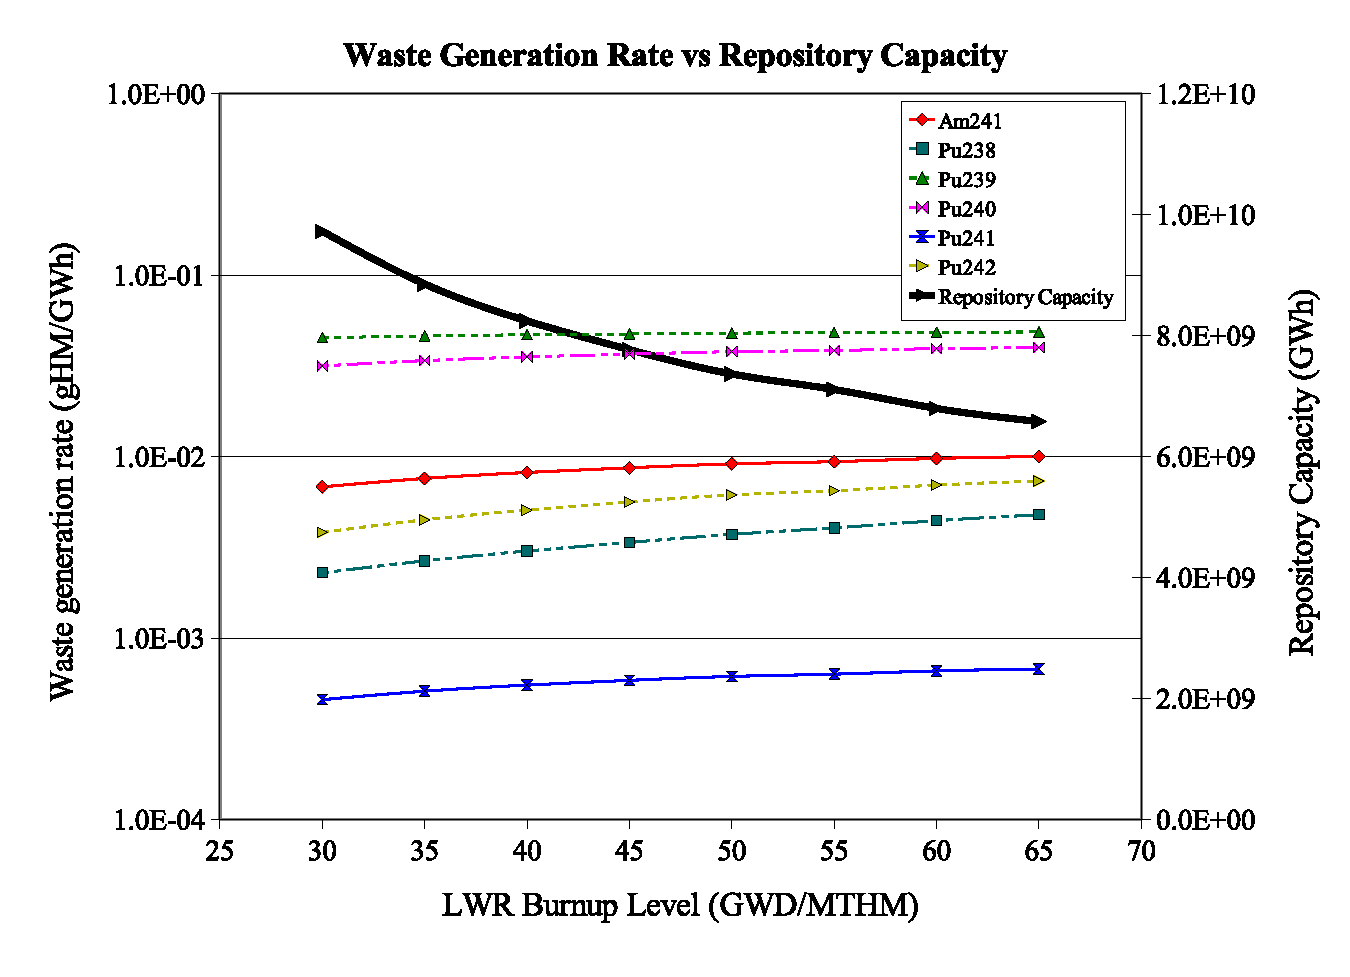
\includegraphics[scale=0.44]{figs/LWR_BUd_sensitivity_RepCap.eps}\FigCaption{Figure 3: Nuclide Generation Rate in the Final Waste}
\end{center}
\end{slide}




%Conclusions
\overlays{3}{
\begin{slide}{Conclusions}
\FromSlide{1}
\begin{itemize}
    \item The sensitivity coefficients let us quantify which input parameters would 
        benefit the most from further parametric studies.

\FromSlide{2}
\vspace{0.75cm}
    \item However, the $S_{\pm x}$ represent linear perturbations that are tied to a base-case scenario.

\FromSlide{3}
\vspace{0.75cm}
    \item To truly move away from base-case scenarios and more deeply study how $R(x)$ behaves
        for all parameters, we need to adopt a more sophisticated methodology...

\FromSlide{1}
\end{itemize}
\end{slide}}




%Ongoing \& Future Work
\overlays{4}{
\begin{slide}{Ongoing \& Future Work}
\FromSlide{1}
\begin{itemize}
    \item We are adopting a stochastic methodology 
        where we simultaneously pick random values for all 30 input parameters.

\vspace{0.2cm}
\FromSlide{2}
    \item Through this method, we obtain tens of thousands of realizations of our fuel cycle model.

\vspace{0.2cm}
\FromSlide{3}
    \item We use \underline{contingency tables} and their corresponding information theoretic measures 
        (\textit{entropy}, \textit{mutual information}, \textit{uncertainty}) to determine the strength of association 
        between all physical inputs and each fuel cycle output.

\vspace{0.2cm}
\FromSlide{4}
    \item Analysis of these measures mimics what we have just seen for $S_{\pm x}$, though
        on a much improved basis.

\FromSlide{1}
\end{itemize}
\end{slide}}



%Ongoing \& Future Work
\overlays{2}{
\begin{slide}{Ongoing \& Future Work}
\FromSlide{1}
\tiny
\begin{center}
\FigCaption{Table 4: Contingency Table for Am/Cm SE to Repository Capacity [PWh]}
\begin{tabular}{|c||c|c|c||c|}
\hline
&$0.9 - 0.99$&$0.99 - 0.999$&$0.999 - 0.9999$&\\
\hline
$300 <$ Rep. Cap. $< 3225$&$4969$&$1159$&$553$&$6681$\\
\hline
$3225 <$ Rep. Cap. $< 6150$&$0$&$2279$&$631$&$2910$\\
\hline
$6150 <$ Rep. Cap. $< 9075$&$0$&$1506$&$914$&$2420$\\
\hline
$9075 <$ Rep. Cap. $< 12000$&$0$&$4$&$2985$&$2989$\\
\hline
&$4969$&$4948$&$5083$&$15000$\\
\hline
\end{tabular}
\end{center}

\FromSlide{2}
\vspace{0.25cm}
Would produce associations such as, 
\begin{center}
\FigCaption{Table 5: Top Parameters Affecting Repository Capacity}
\begin{tabular}{|l|c|}
\hline
\textbf{Parameter $x$}           & \textbf{$U(x|R)$} \\
\hline
\texttt{FR\_SE\_PU}              & 0.085329856138 \\
\hline
\texttt{INT\_SNF\_Storage\_Time} & 0.0592316541992\\
\hline
\texttt{FR\_SE\_AM}              & 0.0403626920053\\
\hline
\texttt{Heat\_Loss\_Factor}      & 0.0168894857328\\
\hline
\texttt{LWR\_SE\_PU}             & 0.0138739809511\\
\hline
\texttt{FR\_TRU\_CR}             & 0.0108559673721\\
\hline
\end{tabular}
\end{center}

\end{slide}}

%Questions
\begin{slide}{Questions}
? ? ? ? ? ? ? ? ? ? ? ? ? ? ? ? ? ? ? ? ? ? ? ? ? ? ? ? ? ? ? 
? ? ? ? ? ? ? ? ? ? ? ? ? ? ? ? ? ? ? ? ? ? ? ? ? ? ? ? ? ? ? 
? ? ? ? ? ? ? ? ? ? ? ? ? ? ? ? ? ? ? ? ? ? ? ? ? ? ? ? ? ? ? 
? ? ? ? ? ? ? ? ? ? ? ? ? ? ? ? ? ? ? ? ? ? ? ? ? ? ? ? ? ? ? 
? ? ? ? ? ? ? ? ? ? ? ? ? ? ? ? ? ? ? ? ? ? ? ? ? ? ? ? ? ? ? 
? ? ? ? ? ? ? ? ? ? ? ? ? ? ? ? ? ? ? ? ? ? ? ? ? ? ? ? ? ? ? 
? ? ? ? ? ? ? ? ? ? ? ? ? ? ? ? ? ? ? ? ? ? ? ? ? ? ? ? ? ? ? 
? ? ? ? ? ? ? ? ? ? ? ? ? ? ? ? ? ? ? ? ? ? ? ? ? ? ? ? ? ? ? 
? ? ? ? ? ? ? ? ? ? ? ? ? ? ? ? ? ? ? ? ? ? ? ? ? ? ? ? ? ? ? 
? ? ? ? ? ? ? ? ? ? ? ? ? ? ? ? ? ? ? ? ? ? ? ? ? ? ? ? ? ? ? 
? ? ? ? ? ? ? ? ? ? ? ? ? ? ? ? ? ? ? ? ? ? ? ? ? ? ? ? ? ? ? 
? ? ? ? ? ? ? ? ? ? ? ? ? ? ? ? ? ? ? ? ? ? ? ? ? ? ? ? ? ? ? 
? ? ? ? ? ? ? ? ? ? ? ? ? ? ? ? ? ?
\end{slide}

\begin{slide}{Bibliography}
\tiny
\begin{enumerate}
    \item \fullcite{Scopatz2009}
    \item \fullcite{Takano1994}
\end{enumerate}
\end{slide}

\end{document}
